%%%% created by (Subramaniyan Neelagandan)

\documentclass[landscape]{slides}
\usepackage[landscape]{geometry}
\usepackage{tikz}
\usepackage{color}
\usepackage{amsfonts}
\usepackage{bm}
%%\usepackage[linesnumbered, ruled, vlined]{algorithm2e}
\usepackage{algorithm}
\usepackage{algpseudocode}
\usepackage{pgfmath}
\usetikzlibrary{shapes.misc,shadows, arrows, shapes, intersections}
\usepackage{geometry}

\geometry{
	left=10mm,
	right=10mm,
	top=5mm,
	bottom=5mm
}

\iffalse

\geometry{
	a4paper,
	total={170mm,257mm},
	left=5mm,
	top=5mm,
}

\fi

\newcommand*\wrapped[1]{\tikz[baseline=(char.base)]{
		\node(char)[draw,fill=white,
		shape=rounded rectangle,
		drop shadow={opacity=.5,shadow xshift=0pt},
		minimum width=1.8cm] (char) {#1};}}

\newcommand*\circled[1]{\tikz[baseline=(char.base)]{
		\node[shape=circle,draw,inner sep=2pt] (char) {#1};}}

\newcommand*\cloud[1]{\tikz[baseline=(char.base)]{
		\node [cloud, draw,cloud puffs=10,cloud puff arc=120,
		aspect=2, inner ysep=1em] (char) {#1};}}


\title{Graph: Clique}
\author{Subramaniyan Neelagandan}
\date{2017-04-09}


\begin{document}

\begin{slide}
	\begin{center}
		{\large Algorithm to find}
	\end{center}
	\begin{itemize}
		\setlength{\itemsep}{0pt}
		\setlength{\parskip}{0pt}
		\setlength{\parsep}{0pt}
		\item Whether graph has clique of given size
		\item Maximum clique size
		\item Number of cliques having maximum size
		\item Enumerate all cliques having maximum size
	\end{itemize}
\end{slide}

\begin{slide}
	\begin{center}
		{\large Algorithm is}
	\end{center}
	\begin{itemize}
		\setlength{\itemsep}{0pt}
		\setlength{\parskip}{0pt}
		\setlength{\parsep}{0pt}
		\item constructive
		\item usable
		\item complete exhaustive search
		\item {$n = |V|$}
		\begin{itemize}
			\item better than quasi-polynomial time \\
			 $ f(n) < \mathcal{O}(n\textsuperscript{{$log{(n)}$} })$ where $n$ is up to few $1000(s)$.
			 \item slower than quasi-polynomial time when $n$ is above few $1000(s)$.
		\end{itemize}
		\item polynomial space complexity - $\mathcal{O}(n\textsuperscript{3})$ where {$n = |V|$}
	\end{itemize}
\end{slide}

\begin{slide}
	\begin{center}
		{\large Relationship between Clique \& Partition}
	\end{center}
	\begin{itemize}
		\setlength{\itemsep}{0pt}
		\setlength{\parskip}{0pt}
		\setlength{\parsep}{0pt}
		\item Each vertex in a clique comes from different partition.
		\item Clique of size {$K$} has vertices from {$K$} different partition.
		\item Number of partitions in a graph can be greater than or equal to maximum clique size of the graph. 
	\end{itemize}
\end{slide}

\begin{slide}
	\begin{center}
		{\large Maximum clique size of {$G$} {\small VS} Maximum clique size for vertex {$v$}}
	\end{center}
	\begin{itemize}
		\setlength{\itemsep}{0pt}
		\setlength{\parskip}{0pt}
		\setlength{\parsep}{0pt}
		\item Let {$G$} be a graph.
		\item Maximum clique size of {$G$} is maximum of maximum clique size of any vertex in {$G$}.
	\end{itemize}
\end{slide}

\begin{slide}
	\begin{center}
		{\large Maximum clique size for vertex {$v$} {\small with respect to} its neighborhood graph }
	\end{center}
	\begin{itemize}
		\setlength{\itemsep}{0pt}
		\setlength{\parskip}{0pt}
		\setlength{\parsep}{0pt}
		\item Let {$G$} be a graph and {$v$} be one of its vertices.
		\item Let {$G'$} be neighborhood graph of {$v$} in {$G$}.
		\item Maximum size of any clique having {$v$} is 1 + maximum clique size of {$G'$}.
	\end{itemize}
\end{slide}

\begin{slide}
\begin{center}
	{\large Neighborhood graph }

	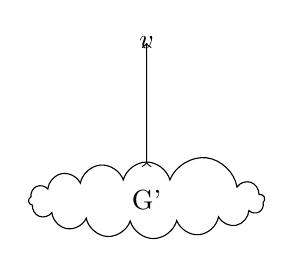
\begin{tikzpicture}
	\node[
	name path=cloud,
	cloud, cloud puffs=15.7,
	minimum width=3cm, draw 
	] (cloud) at (0,0) {G'};
	\path[name path=path21] (cloud.center) -- (0, 2) coordinate (to21);
	\draw[->,
	name intersections={of=cloud and path21,by=from21},
	] 
	(from21) edge node[at end] {$v$} (to21)
	;
	\end{tikzpicture}
\end{center}

	\begin{itemize}
		\setlength{\itemsep}{0pt}
		\setlength{\parskip}{0pt}
		\setlength{\parsep}{0pt}
		\item Let {$G'$} be a graph having maximum clique size {$K$}
		\item Create graph {$G$} by adding vertex {$v$} to {$G'$}.
		\item If {$v$} is connected to all vertices of {$G'$} then maximum clique size of {$G$} is {$K + 1$}.
		\item In other words, {$G'$} being neighborhood graph of vertex {$v$} of graph {$G$}
	\end{itemize}
\end{slide}


\begin{slide}

\begin{center}
	\begin{center}
		{\large Neighborhood graph }
	\end{center}

	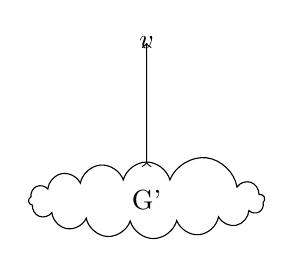
\begin{tikzpicture}
	\node[
	name path=cloud,
	cloud, cloud puffs=15.7,
	minimum width=3cm, draw 
	] (cloud) at (0,0) {G'};
	\path[name path=path21] (cloud.center) -- (0, 2) coordinate (to21);
	\draw[->,
	name intersections={of=cloud and path21,by=from21},
	] 
	(from21) edge node[at end] {$v$} (to21)
	;
	\end{tikzpicture}
\end{center}

	\begin{itemize}
		\setlength{\itemsep}{0pt}
		\setlength{\parskip}{0pt}
		\setlength{\parsep}{0pt}
		\item Let {$G$} be a graph.
		\item Let vertex {$v$} is part of {$G$}.
		\item Let {$K$} be the maximum clique size of vertex {$v$}.
		\item Let {$G'$} be the neighborhood graph of {$v$}.
		\item Maximum clique size of {$G'$} is {$K - 1$}.
		\item If {$v$} is connected to every other vertex in {$G$} then {$G'$} is same as {$G - v$}.
		\item Once maximum clique size of {$v$} is found then we can stop processing further.
	\end{itemize}
\end{slide}

\begin{slide}

\begin{center}
	\begin{center}
		{\large Neighborhood graph }
	\end{center}

	\begin{tikzpicture}
	\node[
	name path=cloud,
	cloud, cloud puffs=15.7,
	minimum width=3cm, draw,
	] (cloud) at (0,0) {G};
	\path[name path=path21] (cloud.center) -- (-3, 3) coordinate (to21);
	\path[name path=path22] (cloud.center) -- (3, 3) coordinate (to22);
	\draw[->,
	name intersections={of=cloud and path21,by=from21},
	name intersections={of=cloud and path22,by=from22},
	] 
	(from21) edge node[at end] {$u$} (to21)
	(from22) edge node[at end] {$v$}  (to22)
	;
	\end{tikzpicture}
\end{center}

	\begin{itemize}
		\setlength{\itemsep}{0pt}
		\setlength{\parskip}{0pt}
		\setlength{\parsep}{0pt}
		\item Let {$G$} be a graph having maximum clique size {$K$}
		\item Create graph {$G$}\textsuperscript{1} by adding vertex {$u$} to {$G$} such that {$u$} is connected to all vertices in {$G$}.
		\item Create graph {$G$}\textsuperscript{2} by adding vertex {$v$} to {$G$} such that {$v$} is connected to all vertices in {$G$}.
		\item Maximum clique size of {$G$}\textsuperscript{1} is {$K + 1$}
		\item Maximum clique size of {$G$}\textsuperscript{2} is {$K + 1$}
		\item Maximum clique size of {$G$}\textsuperscript{1} is equal to maximum clique size of {$G$}\textsuperscript{2}
		\item In other words, if neighborhood graph of vertices {$u$} and {$v$} are same then their maximum clique size is also same.
		\item If vertices {$u$} and {$v$} are part of graph {$H$} and if their neighborhood graph is same then we need to find maximum clique size of neighborhood graph of either vertex {$u$} or vertex {$v$}. 
	\end{itemize}
\end{slide}

\begin{slide}
	\begin{center}
	\begin{center}
		{\large Neighborhood graph }
	\end{center}

		\begin{tikzpicture}
		\node[
		name path=cloud,
		cloud, cloud puffs=15.7,
		minimum width=3cm, draw,
		] (cloud) at (0,0) {G};
		\path[name path=path21] (cloud.center) -- (-3, 3) coordinate (to21);
		\path[name path=path22] (cloud.center) -- (3, 3) coordinate (to22);
		\draw[->,
		name intersections={of=cloud and path21,by=from21},
		name intersections={of=cloud and path22,by=from22},
		] 
		(from21) edge node[at end] {$u$} (to21)
		(from22) edge node[at end] {$v$}  (to22)
		(to21) edge (to22) 
		;
		\end{tikzpicture}
	\end{center}
	
	\begin{itemize}
		\setlength{\itemsep}{0pt}
		\setlength{\parskip}{0pt}
		\setlength{\parsep}{0pt}
		\item Let {$G$} be a graph having maximum clique size {$K$}
		\item Create graph {$G'$} by adding vertex {$u \& v$} to {$G$} such that both {$u \& v$} is connected to all vertices in {$G$}.
		\item Maximum clique size of {$G'$} is {$K + 2$}
		\item Since {$u$} is part of {$v$}'s neighborhood graph and vice versa, we need to find maximum clique for either one.
	\end{itemize}
\end{slide}


\begin{slide}

\begin{center}
	\begin{center}
		{\large Neighborhood graph }
	\end{center}

	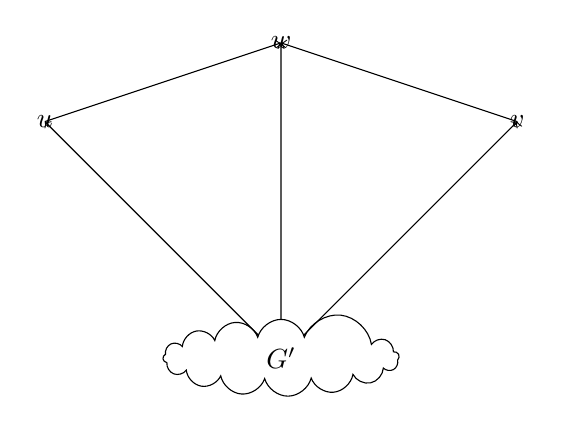
\begin{tikzpicture}
	\node[
	name path=cloud,
	cloud, cloud puffs=15.7,
	minimum width=3cm, draw,
	] (cloud) at (0,0) {{$G'$}};
	\path[name path=path21] (cloud.center) -- (-3, 3) coordinate (to21);
	\path[name path=path22] (cloud.center) -- (3, 3) coordinate (to22);
	\path[name path=path23] (cloud.center) -- (0, 4) coordinate (to23);
	\draw[->,
	name intersections={of=cloud and path21,by=from21},
	name intersections={of=cloud and path22,by=from22},
	name intersections={of=cloud and path23,by=from23}
	] 
	(from21) edge node[at end] {$u$} (to21)
	(from22) edge node[at end] {$v$}  (to22)
	(from23) edge node[at end] {$w$}  (to23)
	(to21) edge (to23)
	(to22) edge (to23)
	;
	\end{tikzpicture}
\end{center}

	\begin{itemize}
		\setlength{\itemsep}{0pt}
		\setlength{\parskip}{0pt}
		\setlength{\parsep}{0pt}
		\item Let {$G$} be a graph.
		\item Let {$u, v \& w$} be one of the vertices of {$G$}.
		\item Let {$G'$} be the subgraph {$G$} without {$u, v \& w$}.
		\item Let {$u, v \& w$} are connected to every vertices in {$G'$}
		\item Let {$u, \& v$} are connected to {$w$}.
		\item In this case {$w$} would be part of neighborhood graph of both {$u, \& v$}.
		\item Maximum size of clique having {$u$} is same as maximum size of clique having {$v$}.
		\item Here, we need to search neighborhood graph of either {$u$} or {$v$} only. Since {$w$} is connected to both {$u, \& v$} and thereby part of {$u, \& v$}'s neighborhood graph, maximum size of clique having {$w$} is same as {$u$} or {$v$}.
	\end{itemize}
\end{slide}

\begin{slide}
	\begin{center}
		{\large Active neighborhood graph }
	\end{center}

	\begin{itemize}
		\setlength{\itemsep}{0pt}
		\setlength{\parskip}{0pt}
		\setlength{\parsep}{0pt}
		\item Let {$G$} be a graph.
		\item Let {$V$} be set of vertices of {$G$}.
		\item Let {$V$}\textsuperscript{1} be the set of vertices of {$V$} which are already searched for the maximum clique.
		\item Let {$V$}\textsuperscript{2} be the set of vertices of {$V$} not in {$V$}\textsuperscript{1}. {$V\textsuperscript{2} = \{V - V\textsuperscript{1}\}$}.
		\item Members of {$V$}\textsuperscript{2} are not yet searched.
		\item Let vertex {$v$} be one of the vertices of {$V$}\textsuperscript{2}.
		\item Let the neighborhood graph created for vertex {$v$} to search be {$G$}\textsuperscript{1}.
		\item It is enough to restrict the members of {$G$}\textsuperscript{1} be the vertices from {$V$}\textsuperscript{2}. No need to consider members of {$V$}\textsuperscript{1}.
		\item Now, if there exists a vertex {$u$} of {$V$}\textsuperscript{1} whose neighborhood graph is superset of {$G$}\textsuperscript{1} then we don't need to search.
	\end{itemize}
\end{slide}


\begin{slide}
	\begin{center}
		{\large Recursion depth }
	\end{center}
	
	\begin{itemize}
		\setlength{\itemsep}{0pt}
		\setlength{\parskip}{0pt}
		\setlength{\parsep}{0pt}
		\item Recursion depth never exceeds maximum clique size of the given graph $G$ when using neighborhood search.
	\end{itemize}
\end{slide}


\begin{slide}
	\begin{center}
		{\large Partition extraction }
	\end{center}

	\begin{itemize}
		\setlength{\itemsep}{0pt}
		\setlength{\parskip}{0pt}
		\setlength{\parsep}{0pt}
		\item Let {$G$} be a graph.
		\item Let {$v$} be a vertex of {$G$}.
		\item If {$v$} is connected to every other vertex in this graph {$G$}, then maximum clique size of {$G$} is 1 + maximum clique size of {$\{ G - v\}$}.
	\end{itemize}
\end{slide}

\begin{slide}
	\begin{center}
		{\large Partition extraction }
	\end{center}

	\begin{itemize}
		\setlength{\itemsep}{0pt}
		\setlength{\parskip}{0pt}
		\setlength{\parsep}{0pt}
		\item Let {$G$} be a graph.
		\item Let {$V$} be all vertices of {$G$}.
		\item Let {$v$} be a vertex of graph {$G$}.
		\item Let {$V$}\textsuperscript{1} be the set of vertices to which {$v$} is not connected.
		\item Let {$V$}\textsuperscript{2} be {$\{ V\textsuperscript{1} + v \}$}.
		\item Let {$V$}\textsuperscript{3} be {$\{ V - V\textsuperscript{2}\}$}.
		\item Let {$G$}\textsuperscript{1} be induced graph of {$G$} containing all vertices of {$V$}\textsuperscript{3} only.
		\item Now, if vertex {$v$} is connected to all vertices in {$V$}\textsuperscript{3} then {$G$}\textsuperscript{1} becomes neighborhood graph of {$v$}.
		\item In addition, if all vertices in {$V$}\textsuperscript{2} are independant and forms a partition, then maximum clique size of {$G$} is 1 + maximum clique size of {$G$}\textsuperscript{1}.
		\item In this case, we can skip searching neighborhood graph of all vertices of {$V$}\textsuperscript{1}.
	\end{itemize}
\end{slide}



\begin{slide}
	\begin{tikzpicture}
	\def\n{11}
	
	\node[draw,circle,inner sep=2pt] at (0, \n * 1.5) {$v$};

	\foreach \y in {1,...,\n}{
		\node[draw,circle,inner sep=2pt] at (0, \y * 1.5) {$v$};
	}
	
	\foreach \y in {1,...,\n}{
		\node[draw,circle,inner sep=2pt] at (\y * 2, \n * 1.5) {$v$};
	}

	\draw[dotted] (0, 1.5) -- node[right] {$G'$} (0, \n * 1.5);
	\end{tikzpicture}
\end{slide}


\begin{slide}
	\begin{center}
	{\large{Top-down processing \\ (Partition Extraction)}}
	\end{center}

	\begin{itemize}
		\setlength{\itemsep}{0pt}
		\setlength{\parskip}{0pt}
		\setlength{\parsep}{0pt}
		\item If a partition {$P$} can be extracted from active graph {$G"$} then extract the partition.
		\item Increment count of partitions found.
		\item Reduce active graph {$G"$} to {$G" - P$}.
		\item Repeat until there is no more partition to be extracted. 
	\end{itemize}
\end{slide}

\begin{slide}
	\begin{center}
		{\large{Bottom-up processing \\ (Neighborhood graph duplicate elimination)}}
	\end{center}

	Once neighborhood graph search is complete then 
	\begin{itemize}
		\setlength{\itemsep}{0pt}
		\setlength{\parskip}{0pt}
		\setlength{\parsep}{0pt}
		\item Remove the vertex {$v$} whose neighborhood graph is explored from active graph.
		\item Remove any vertex {$u$} part of active graph that has same neighborhood graph as {$v$}.
		\item Repeat this process for each vertex {$v$} that is removed till there is no more vertex to be removed.
	\end{itemize}
\end{slide}

\begin{slide}
	\begin{center}
		{\large{Creating neighborhood graph of vertex {$v$}}}
	\end{center}

	\begin{itemize}
		\setlength{\itemsep}{0pt}
		\setlength{\parskip}{0pt}
		\setlength{\parsep}{0pt}
		\item if the search is for maximum clique then neighborhood graph is subgraph of {$G$} containing list of vertices to which {$v$} is connected.
		\item If the search is for a specific clique size {$K$} then neighborhood graph is subgraph of {$G$} containing list of vertices to which {$v$} is connected and have at least {$K - 1$} edges.
	\end{itemize}
\end{slide}


\begin{slide}
	\begin{center}
		{\large Active neighborhood graph search }
	\end{center}

	{\large Ensure that neighborhood graph that needs to be searched is not same or subset of already searched vertex's neighborhood graph}
\end{slide}


\begin{algorithm}
	\caption{$FindMaximumCliqueSize$ : O(n\textsuperscript{$n$})}
	\begin{algorithmic}[1]
	\Function{FindMaximumCliqueSize}{$G(V,E)$}
		\State $kMax \gets 0$
		\ForAll{($v$ in $V$)}
			\State $G' \gets neighborhood(G, v)$
			\State $kMax_1 \gets FindMaximumCliqueSize(G')$
			\If{(($kMax_1 + 1) > kMax)$)}
				\State $kMax \gets kMax_1 + 1$
			\EndIf
		\EndFor
		\State \textbf{return} $kMax$
	\EndFunction
	\end{algorithmic}
\end{algorithm}

\begin{algorithm}
	\caption{$FindMaximumCliqueSize$ : O(n!)}
	\begin{algorithmic}[1]
		\Function{FindMaximumCliqueSize}{$G(V,E)$}
		\State $kMax \gets 0$
		\State {\color{red} $H \gets G$}
		\ForAll{($v$ in $V$)}
			\State $G' \gets neighborhood({\color{red} H}, v)$
			\State $kMax_1 \gets FindMaximumCliqueSize(G')$
			\If{(($kMax_1 + 1) > kMax)$)}
				\State $kMax \gets kMax_1 + 1$
			\EndIf
			\State {\color{red} $H \gets \{H - v\}$}
		\EndFor
		\State \textbf{return} $kMax$
		\EndFunction
	\end{algorithmic}
\end{algorithm}

\begin{algorithm}
	\caption{$FindMaximumCliqueSize$ : O(n!)}
	\begin{algorithmic}[1]
		\Function{FindMaximumCliqueSize}{$G(V,E), k$}
		\State $kMax \gets {\color{red}max(k - 1, 0)}$
		\State $H \gets G$
		\ForAll{($v$ in $V$)}
			\State $G' \gets neighborhood(H, v, {\color{red}kMax})$
			{\color{red} \If{($|G'| >= kMax$)}
				\State $(found_1, kMax_1) \gets FindMaximumCliqueSize(G', kMax)$
				\If{($found_1$ and (($kMax_1 + 1) > kMax$))}
					\State $kMax \gets kMax_1 + 1$
				\EndIf
			\EndIf }
			\State $H \gets \{H - v\}$
		\EndFor
		\State \textbf{return} {\color{red} $(kMax >= k, kMax)$ }
		\EndFunction
	\end{algorithmic}
\end{algorithm}


\begin{slide}
	\begin{center}
		{\large Complete multipartite graph }
	\end{center}
	
	\begin{itemize}
		\setlength{\itemsep}{0pt}
		\setlength{\parskip}{20pt}
		\setlength{\parsep}{0pt}
		\item  A complete multipartite graph is a graph that is complete {$k$}-partite for some {$k$}.
		\item A complete {$k$}-partite graph is a {$k$}-partite graph in which there is an edge between every pair of vertices from different independent sets.
	\end{itemize}
\end{slide}


\begin{slide}
	\begin{center}{
		\normalsize{
			A complete 6-partite sample graph $K_2,_2,_2,_2,_2,_2$ \\ \hfill \break
			$G$=\{$v_{1:1},v_{1:2},v_{2:1},v_{2:2},v_{3:1},v_{3:2},v_{4:1},v_{4:2},v_{5:1},v_{5:2},v_{6:1},v_{6:2}$\} \\
			\hfill \break
		}
		\wrapped{\large{$\{v_{1:1}, v_{1:2}\}$}} 	\\ \hfill \break
		\wrapped{\large{$\{v_{2:1}, v_{2:2}\}$}}	\\ \hfill \break
		\wrapped{\large{$\{v_{3:1}, v_{3:2}\}$}}	\\ \hfill \break
		\wrapped{\large{$\{v_{4:1}, v_{4:2}\}$}}	\\ \hfill \break
		\wrapped{\large{$\{v_{5:1}, v_{5:2}\}$}}	\\ \hfill \break
		\wrapped{\large{$\{v_{6:1}, v_{6:2}\}$}}	\\ \hfill \break
	}
	\end{center}
\end{slide}

\begin{slide}
\begin{itemize}
	\setlength{\itemsep}{0pt}
	\setlength{\parskip}{20pt}
	\setlength{\parsep}{0pt}
	\item Time complexity : $f(x) = 2\textsuperscript{6} + 2\textsuperscript{5} + 2\textsuperscript{4} + $
	\item Number of distinct cliques of size 6 is $2\textsuperscript{6}$
	\item Space to store $2\textsuperscript{6}$ 6-cliques is $|V|$
\end{itemize}
\end{slide}


\begin{slide}
	\begin{center}{
			\normalsize{
			A complete 6-partite sample graph $K_3,_3,_3,_3,_3,_3$ \\ \hfill \break
				$G$=\{$v_{1:1},v_{1:2},v_{1:3},v_{2:1},v_{2:2},v_{2:3},v_{3:1},v_{3:2},v_{3:3},$ \\
				$v_{4:1},v_{4:2},v_{4:3},v_{5:1},v_{5:2},v_{5:3},v_{6:1},v_{6:2},v_{6:3}$\} \\
				\hfill \break
			}
			\wrapped{\large{$\{v_{1:1}, v_{1:2}, v_{1:3}\}$}} 	\\ \hfill \break
			\wrapped{\large{$\{v_{2:1}, v_{2:2}, v_{2:3}\}$}}	\\ \hfill \break
			\wrapped{\large{$\{v_{3:1}, v_{3:2}, v_{3:3}\}$}}	\\ \hfill \break
			\wrapped{\large{$\{v_{4:1}, v_{4:2}, v_{4:3}\}$}}	\\ \hfill \break
			\wrapped{\large{$\{v_{5:1}, v_{5:2}, v_{5:3}\}$}}	\\ \hfill \break
			\wrapped{\large{$\{v_{6:1}, v_{6:2}, v_{6:3}\}$}}
		}
	\end{center}
\end{slide}

\begin{slide}
\begin{itemize}
	\setlength{\itemsep}{0pt}
	\setlength{\parskip}{20pt}
	\setlength{\parsep}{0pt}
	\item Time complexity : $f(x) = 3\textsuperscript{6} + 3\textsuperscript{5} + 3\textsuperscript{4} + 3\textsuperscript{3} + $
	\item Number of distinct cliques of size 6 is $3\textsuperscript{6}$
	\item Space to store $3\textsuperscript{6}$ 6-cliques is $|V|$
\end{itemize}
\end{slide}


\begin{algorithm}
	\caption{$FindMaximumCliqueSize$ : O(exp\textsuperscript{(f(n))})}
	\begin{algorithmic}[1]
		\Function{FindMaximumCliqueSize}{$G(V,E), k$}
		\State $kMax \gets max(k - 1, 0)$
		\State {\color{red} $partitions \gets \{\}$}
		\State $H \gets G$
		\While{$(|H| > kMax)$}
			{\color{red} \While{$|(p := ExtractPartition(H))| > 0$}
				\State $partitions \gets partitions \cup p$
				\State $H \gets H - p$
				\State $kMax \gets max(kMax - 1, 0$)
			\EndWhile
			\If{($H = \{\}$)}
				\State \textbf{break}
			\EndIf }
			\State $v \gets PickAVertex(H)$
			\State $G' \gets neighborhood(H, v, kMax)$
		\algstore{algsave}
	\end{algorithmic}
\end{algorithm}

\begin{algorithm}
	\begin{algorithmic}[1]
		\algrestore{algsave}
			\If{($|G'| >= kMax$)}
				\State $(found_1, kMax_1) \gets FindMaximumCliqueSize(G', kMax)$
				\If{($found_1$ and (($kMax_1 + 1) > kMax$))}
				\State $kMax \gets kMax_1 + 1$
			\EndIf
		\EndIf
		\State $H \gets \{H - v\}$
		\EndWhile
		\State {\color{red} $kMax \gets |partitions| + kMax$ }
		\State \textbf{return} $(kMax >= k, kMax)$
		\EndFunction
	\end{algorithmic}
\end{algorithm}

\clearpage
\begin{slide}
	\begin{center}{\large Top-down }\end{center}
	\begin{itemize}
		\setlength{\itemsep}{0pt}
		\setlength{\parskip}{20pt}
		\setlength{\parsep}{0pt}
		\item The above algorithm uses top-down optimization.
		\item Time complexity is $O(n\textsuperscript{3})$ for complete multipartite graphs.
		\item Still not good enough for random graph.
	\end{itemize}
\end{slide}


\begin{algorithm}
	\caption{$FindMaximumCliqueSize$ : O(exp\textsuperscript{(f(n))})}
	\begin{algorithmic}[1]
		\Function{FindMaximumCliqueSize}{$G(V,E), k$}
		\State $kMax \gets max(k - 1, 0)$
		\State $H \gets G$
		\While{$(|H| > kMax)$}
			\State $v \gets PickAVertex(H)$
			\State $G' \gets neighborhood(H, v, kMax)$
			\If{($|G'| >= kMax$)}
				\State $(found_1, kMax_1) \gets FindMaximumCliqueSize(G', kMax)$
				\If{($found_1$ and (($kMax_1 + 1) > kMax$))}
					\State $kMax \gets kMax_1 + 1$
				\EndIf
			\EndIf
		\algstore{algsave}
	\end{algorithmic}
\end{algorithm}


\begin{algorithm}
	\begin{algorithmic}[1]
		\algrestore{algsave}
			\State {\color{red} $G' \gets neighborhood(H, v)$ }
			\State $H \gets \{H - v\}$
			{\color{red}
			\ForAll {$v' \in H$}
				\State $G'' \gets neighborhood(H, v')$
				\If{($isSubgraph(G', G'')$}
					\State $H \gets \{H - v'\}$
				\EndIf
			\EndFor }
		\EndWhile
		\State \textbf{return} $(kMax >= k, kMax)$
		\EndFunction
	\end{algorithmic}
\end{algorithm}


\begin{algorithm}
	\caption{$FindMaximumCliqueSize$ : O(exp\textsuperscript{(f(n))})}
	\begin{algorithmic}[1]
		\Function{FindMaximumCliqueSize}{$G(V,E), k$}
		\State $kMax \gets max(k - 1, 0)$
		\State $H \gets G$
		\While{$(|H| > kMax)$}
		\State $v \gets PickAVertex(H)$
		\State $G' \gets neighborhood(H, v, kMax)$
		\If{($|G'| >= kMax$)}
			{\color{red}
			\State $search \gets true$
			\ForAll {$v' \in \{G - H\}$}
				\State $G'' \gets neighborhood(G, v')$
				\If{($isSubgraph(G'', G')$}
					\State $search \gets false$
				\EndIf
			\EndFor }
			\If {$search$}
				\State $(found_1, kMax_1) \gets FindMaximumCliqueSize(G', kMax)$
		\algstore{algsave}
	\end{algorithmic}
\end{algorithm}


\begin{algorithm}
	\begin{algorithmic}[1]
		\algrestore{algsave}
				\If{($found_1$ and (($kMax_1 + 1) > kMax$))}
					\State $kMax \gets kMax_1 + 1$
				\EndIf
			\EndIf
		\EndIf
		\State $G' \gets neighborhood(H, v)$
		\State $H \gets \{H - v\}$
		
		\ForAll {$v' \in H$}
		\State $G'' \gets neighborhood(H, v')$
		\If{($isSubgraph(G', G'')$}
		\State $H \gets \{H - v'\}$
		\EndIf
		\EndFor
		\EndWhile
		\State \textbf{return} $(kMax >= k, kMax)$
		\EndFunction
	\end{algorithmic}
\end{algorithm}


\clearpage
\begin{slide}
	\begin{center}{\large Bottom-up }\end{center}
	\begin{itemize}
		\setlength{\itemsep}{0pt}
		\setlength{\parskip}{20pt}
		\setlength{\parsep}{0pt}
		\item The above algorithm uses bottom-up optimization.
		\item Time complexity is $O(n\textsuperscript{3})$ for complete multipartite graphs.
		\item Still not good enough for random graph.
	\end{itemize}
\end{slide}


\begin{algorithm}
	\caption{$FindMaximumCliqueSize$ : O(exp\textsuperscript{(f(n))})}
	\begin{algorithmic}[1]
		\Function{FindMaximumCliqueSize}{$G(V,E), k$}
		\State $kMax \gets max(k - 1, 0)$
		\State $partitions \gets \{\}$
		\State $H \gets G$
		\While{$(|H| > kMax)$}
			\While{$|(p := ExtractPartition(H))| > 0$}
				\State $partitions \gets partitions \cup p$
				\State $H \gets H - p$
				\State $kMax \gets max(kMax - 1, 0$)
			\EndWhile
			\If{($H = \{\}$)}
				\State \textbf{break}
			\EndIf
			\State $v \gets PickAVertex(H)$
			\State $G' \gets neighborhood(H, v, kMax)$
			\If{($|G'| >= kMax$)}
				\State $search \gets true$
		\algstore{algsave}
	\end{algorithmic}
\end{algorithm}


\begin{algorithm}
	\begin{algorithmic}[1]
		\algrestore{algsave}
				\ForAll {$v' \in \{G - H\}$}
					\State $G'' \gets neighborhood(G, v')$
						\If{($isSubgraph(G'', G')$}
							\State $search \gets false$
						\EndIf
					\EndFor
					\If {$search$}
						\State $(found_1, kMax_1) \gets FindMaximumCliqueSize(G', kMax)$
						\If{($found_1$ and (($kMax_1 + 1) > kMax$))}
							\State $kMax \gets kMax_1 + 1$
						\EndIf
					\EndIf
				\EndIf
				\State $G' \gets neighborhood(H, v)$
				\State $H \gets \{H - v\}$
			
				\ForAll {$v' \in H$}
					\State $G'' \gets neighborhood(H, v')$
					\If{($isSubgraph(G', G'')$}
						\State $H \gets \{H - v'\}$
					\EndIf
		\algstore{algsave}
	\end{algorithmic}
\end{algorithm}


\begin{algorithm}
	\begin{algorithmic}[1]
		\algrestore{algsave}
				\EndFor
			\EndWhile
			\State $kMax \gets |partitions| + kMax$
			\State \textbf{return} $(kMax >= k, kMax)$
		\EndFunction
	\end{algorithmic}
\end{algorithm}

\clearpage

\begin{slide}
	\begin{center}{\large Top-down with Bottom-up }\end{center}
	\begin{itemize}
		\setlength{\itemsep}{0pt}
		\setlength{\parskip}{20pt}
		\setlength{\parsep}{0pt}
		\item The above algorithm uses top-down with bottom-up optimization.
		\item Time complexity is $O(n\textsuperscript{3})$ for complete multipartite graphs.
		\item Still not good enough for random graph.
	\end{itemize}
\end{slide}

\begin{slide}
	\begin{center}{\large Vertex selection (PickAVertex) }\end{center}
	\begin{itemize}
		\setlength{\itemsep}{0pt}
		\setlength{\parskip}{20pt}
		\setlength{\parsep}{0pt}
		\item Picking a vertex with largest degree.
		\item Picking a vertex with least degree.
	\end{itemize}
\end{slide}


\begin{algorithm}
	\caption{$FindMaximumCliqueSize$ : O(exp\textsuperscript{(f(n))})}
	\begin{algorithmic}[1]
		\Function{FindMaximumCliqueSize}{$G(V,E), k$}
		\State $kMax \gets max(k - 1, 0)$
		\State $partitions \gets \{\}$
		\State $H \gets G$
		\While{$(|H| > kMax)$}
		\While{$|(p := ExtractPartition(H))| > 0$}
		\State $partitions \gets partitions \cup p$
		\State $H \gets H - p$
		\State $kMax \gets max(kMax - 1, 0$)
		\EndWhile
		\If{($H = \{\}$)}
		\State \textbf{break}
		\EndIf
		\State $v \gets {\color{red} PickAVertexWithLargestDegree(H)}$
		\State $G' \gets neighborhood(H, v, kMax)$
		\If{($|G'| >= kMax$)}
		\State $search \gets true$
		\ForAll {$v' \in \{G - H\}$}
		\algstore{algsave}
	\end{algorithmic}
\end{algorithm}


\begin{algorithm}
	\begin{algorithmic}[1]
		\algrestore{algsave}
		\State $G'' \gets neighborhood(G, v')$
		\If{($isSubgraph(G'', G')$}
		\State $search \gets false$
		\EndIf
		\EndFor
		\If {$search$}
		\State $(found_1, kMax_1) \gets FindMaximumCliqueSize(G', kMax)$
		\If{($found_1$ and (($kMax_1 + 1) > kMax$))}
		\State $kMax \gets kMax_1 + 1$
		\EndIf
		\EndIf
		\EndIf
		\State $G' \gets neighborhood(H, v)$
		\State $H \gets \{H - v\}$
		
		\ForAll {$v' \in H$}
			\State $G'' \gets neighborhood(H, v')$
			\If{($isSubgraph(G', G'')$}
				\State $H \gets \{H - v'\}$
			\EndIf
		\EndFor
		\algstore{algsave}
	\end{algorithmic}
\end{algorithm}


\begin{algorithm}
	\begin{algorithmic}[1]
		\algrestore{algsave}
		\EndWhile
		\State $kMax \gets |partitions| + kMax$
		\State \textbf{return} $(kMax >= k, kMax)$
		\EndFunction
	\end{algorithmic}
\end{algorithm}

\clearpage

\begin{slide}
	\begin{center}{\large Top-down with Bottom-up: picking vertex with largest degree}\end{center}
	\begin{itemize}
		\setlength{\itemsep}{0pt}
		\setlength{\parskip}{20pt}
		\setlength{\parsep}{0pt}
		\item Time complexity is $O(exp\textsuperscript{(f(n))})$ for random graphs.
		\item Time complexity for picking random vertex is worst case time complexity of picking either largest degree or least degree vertex for search. In this case, picking a vertex with largest degree.
	\end{itemize}
\end{slide}


\begin{algorithm}
	\caption{$FindMaximumCliqueSize$ : O(n\textsuperscript{(log(n))})}
	\begin{algorithmic}[1]
		\Function{FindMaximumCliqueSize}{$G(V,E), k$}
		\State $kMax \gets max(k - 1, 0)$
		\State $partitions \gets \{\}$
		\State $H \gets G$
		\While{$(|H| > kMax)$}
		\While{$|(p := ExtractPartition(H))| > 0$}
		\State $partitions \gets partitions \cup p$
		\State $H \gets H - p$
		\State $kMax \gets max(kMax - 1, 0$)
		\EndWhile
		\If{($H = \{\}$)}
		\State \textbf{break}
		\EndIf
		\State $v \gets {\color{red} PickAVertexWithLeastDegree(H)}$
		\State $G' \gets neighborhood(H, v, kMax)$
		\If{($|G'| >= kMax$)}
		\State $search \gets true$
		\ForAll {$v' \in \{G - H\}$}
		\algstore{algsave}
	\end{algorithmic}
\end{algorithm}


\begin{algorithm}
	\begin{algorithmic}[1]
		\algrestore{algsave}
		\State $G'' \gets neighborhood(G, v')$
		\If{($isSubgraph(G'', G')$}
		\State $search \gets false$
		\EndIf
		\EndFor
		\If {$search$}
		\State $(found_1, kMax_1) \gets FindMaximumCliqueSize(G', kMax)$
		\If{($found_1$ and (($kMax_1 + 1) > kMax$))}
		\State $kMax \gets kMax_1 + 1$
		\EndIf
		\EndIf
		\EndIf
		\State $G' \gets neighborhood(H, v)$
		\State $H \gets \{H - v\}$
		
		\ForAll {$v' \in H$}
		\State $G'' \gets neighborhood(H, v')$
		\If{($isSubgraph(G', G'')$}
			\State $H \gets \{H - v'\}$
		\EndIf
		\EndFor
		\algstore{algsave}
	\end{algorithmic}
\end{algorithm}


\begin{algorithm}
	\begin{algorithmic}[1]
		\algrestore{algsave}
		\EndWhile
		\State $kMax \gets |partitions| + kMax$
		\State \textbf{return} $(kMax >= k, kMax)$
		\EndFunction
	\end{algorithmic}
\end{algorithm}

\clearpage

\begin{slide}
	\begin{center}{\large Top-down with Bottom-up: picking vertex with least degree}\end{center}
	\begin{itemize}
		\setlength{\itemsep}{0pt}
		\setlength{\parskip}{20pt}
		\setlength{\parsep}{0pt}
		\item Time complexity is better than $O(n\textsuperscript{log\textsuperscript{n}})$ for random graphs with $n$ up to few 1000(s). Slower than this when $n$ is above few 1000(s).
	\end{itemize}
\end{slide}

\begin{slide}
	\begin{center}{\large WHY?}\end{center}
\end{slide}


\begin{slide}
	\begin{tikzpicture}
	\draw (-1.5,0) parabola (-6,10);
	\draw (1.5,0) parabola (6,10);
	\draw (-1.5,0) -- (1.5,0); 
	\draw (-6,10) -- node[above] {$largest |d|$} (6,10); 
	\end{tikzpicture}
	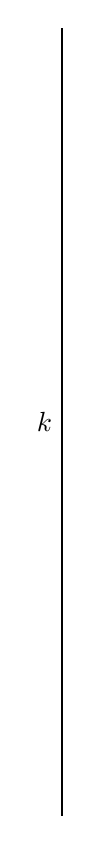
\begin{tikzpicture}
	\draw (0,10) -- node[left] {$k$} (0,0); 
	\end{tikzpicture}
	\begin{tikzpicture}
	\foreach \sgn in {-,+}
	\draw plot[domain=6:10] ({\sgn 1/20*(\x*\x)},\x);
	\draw (-5,10) -- node[above] {$least |d|$} (5,10); 
	\draw (0,0) -- node[right] {$k'$} (0,6);
	\draw ({-(6*6)/20},6) -- ({(6*6)/20},6);
	\end{tikzpicture}
	\small{
	\begin{itemize}
	\setlength{\itemsep}{0pt}
	\setlength{\parskip}{20pt}
	\setlength{\parsep}{0pt}
	\item $k$ is maximum clique size of graph $G$.
	\item At depth ($k - k'$), both top-down and bottom-up gets triggered aggressively and reducing further levels.
	\end{itemize}
	}
\end{slide}


\begin{slide}
	\begin{tikzpicture}
	\draw (-1.5,0) parabola (-6,10);
	\draw (1.5,0) parabola (6,10);
	\draw (-1.5,0) -- (1.5,0); 
	\draw (-6,10) -- node[above] {$largest |d|$} (6,10); 
	\end{tikzpicture}
	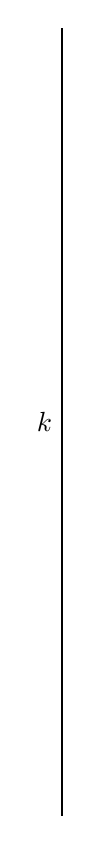
\begin{tikzpicture}
	\draw (0,10) -- node[left] {$k$} (0,0); 
	\end{tikzpicture}
	\begin{tikzpicture}
	\foreach \sgn in {-,+}
	\draw plot[domain=6:10] ({\sgn 1/20*(\x*\x)},\x);
	\draw (-5,10) -- node[above] {$least |d|$} (5,10); 
	\draw (0,0) -- node[right] {$k'$} (0,6);
	\draw ({-(6*6)/20},6) -- node[above] {$n' < 2k'$} ({(6*6)/20},6);
	\end{tikzpicture}
\end{slide}


\begin{slide}
	\begin{center}{\large Hot spots}\end{center}
	\begin{itemize}
		\setlength{\itemsep}{0pt}
		\setlength{\parskip}{20pt}
		\setlength{\parsep}{0pt}
		\item Checking each neighbor vertex has at least clique-size common neighbors.
		\item Neighborhood graph generation
		\item Working set involved in bottom-up (collapsing identical processed neighborhood graph) processing.
		\item Recursion depth
	\end{itemize}
\end{slide}


\begin{slide}
	\begin{center}{\large Picking vertex with largest degree}\end{center}
	\small
	\begin{itemize}
		\setlength{\itemsep}{0pt}
		\setlength{\parskip}{20pt}
		\setlength{\parsep}{0pt}
		\item Convergence of vertices in neighborhood graph at each level to searching clique size is slow.
		\item Vertices to be explored at each level is maximum possible.
		\item Depth of the recursion is almost equal to maximum clique size of the graph.
		\item Hit ratio of top-down (partition extraction) and bottom-up (collapse of identical neighborhood graph) are moderate.
		\item Bottom-up processing needs to process larger set which leads to higher time consumption.
		\item Pretty much all hot spots are affected negatively to the maximum.
	\end{itemize}
\end{slide}


\begin{slide}
	\begin{tikzpicture}
	\draw[loosely dotted] (0,4) -- node[above] {$k$} (18,4); 
	\draw[dashed] (0,11) -- (15,4); 
	\draw[loosely dashed] (15,4) -- (18,3); 
	\draw[red] (0,11) -- (4,8.2);
	\draw[red] (4,8.2) -- (9,4);
	\draw (0,0) -- node[left] {$d$} (0,13); 
	\draw (0,0) -- node[below] {$|V|$} (20,0); 
	\draw[line width=1mm, ->] (0.2,8) -- (0.2,6); 
	\draw[line width=1mm, ->] (8,0.2) -- (10,0.2); 
	\end{tikzpicture}
\end{slide}



\begin{slide}
	\begin{center}{\large Picking vertex with least degree}\end{center}
	\begin{itemize}
		\setlength{\itemsep}{0pt}
		\setlength{\parskip}{20pt}
		\setlength{\parsep}{0pt}
		\item Convergence of vertices in neighborhood graph at each level to searching clique size is aggressive.
		\item Iterations at each level is as small as possible.
		\item Vertices which does not have enough neighbors to produce clique of given size are removed without further processing.
		\item Hit ratio of top-down (partition extraction) and bottom-up (collapse of identical neighborhood graph) are aggressive.
		\item Bottom-up processing needs to process smaller set which leads to lower time consumption.
		\item Quicker convergence leads to denser neighborhood graph at inner recursion levels. This lets top-down (partition extraction) processing possible. Since every partition is a level, every extraction leads to reduction in levels needs to be explored.
		\item Pretty much all hot spots are affected positively to the minimum.
	\end{itemize}
\end{slide}

\begin{slide}
	\begin{tikzpicture}
	\draw[loosely dotted] (0,4) -- node[above] {$k$} (18,4); 
	\draw[dashed] (0,11) -- (18,8); 
	\draw[red] (4,4) -- (14,7.5);
	\draw[red] (14,7.5) -- (18,8);
	\draw (0,0) -- node[left] {$d$} (0,13); 
	\draw (0,0) -- node[below] {$|V|$} (20,0); 
	\draw[line width=1mm, ->] (0.2,8) -- (0.2,6); 
	\draw[line width=1mm, <-] (8,0.2) -- (10,0.2); 
	\end{tikzpicture}
\end{slide}


\begin{slide}
	\centering
	\begin{tikzpicture}
	\draw[loosely dotted] (0,4) -- node[above] {$k$} (18,4); 
	\draw[dashed] (0,11) -- (15,4); 
	\draw[loosely dashed] (15,4) -- (18,3); 
	\draw[red] (13.6,4) arc [x radius=5.6, y radius=3, start angle=31, end angle=150];
	\draw (0,0) -- node[left] {$d$} (0,13); 
	\draw (0,0) -- node[below] {$|V|$} (20,0); 
	\draw[line width=1mm, ->] (0.2,8) -- (0.2,6); 
	\draw[line width=1mm, <-] (8,0.2) -- (10,0.2); 
	\end{tikzpicture}
\end{slide}


\begin{slide}
	\begin{tikzpicture}
	\draw[loosely dotted] (0,4) -- node[above] {$k$} (18,4); 
	\draw[dashed] (0,11) -- (15,4); 
	\draw[red] (14.8,4) arc [x radius=8.2, y radius=3, start angle=48, end angle=130];
	\draw (0,0) -- node[left] {$d$} (0,13); 
	\draw (0,0) -- node[below] {$|V|$} (20,0); 
	\draw[line width=1mm, ->] (0.2,8) -- (0.2,6); 
	\draw[line width=1mm, <-] (8,0.2) -- (10,0.2); 
	\end{tikzpicture}
\end{slide}


\begin{slide}
	\begin{center}{\large Finding Clique of $k$ size in graph $G$ with $n < 2k$}\end{center}
	\begin{itemize}
		\setlength{\itemsep}{0pt}
		\setlength{\parskip}{20pt}
		\setlength{\parsep}{0pt}
		\item Sort vertices by degree in descending order.
		\item Place top $k$ vertices in set $S_1$.
		\item place rest of the vertices in set $S_2$.
		\item Let $C_1$ be sum of edges of vertices in set $S_1$.
		\item Let $C_2$ be the sum of edges of vertices in set $S_2$.
		\item Let $k'$ ($k' < k$) be the number of vertices in set $S_2$.
		\item Let $E_1$ = $C_1$ - ($k$($k - 1$))/2.
		\item Let $E_2$ = $C_2$ - ($k'$($k' - 1$))/2.
		\item At least $E_1$ edges of $S_1$ vertices are connected to $S_2$ vertices.
		\item At least $E_2$ edges of $S_2$ vertices are connected to $S_1$ vertices.
		\item Actual number of edges that connects vertices from $S_1$ with $S_2$ are at least $E_1$.
		\item Actual number of edges that connects vertices from $S_1$ with $S_2$ are exactly $E_1$ when $S_1$ has clique of $k$.
		\item Actual number of edges that connects vertices from $S_2$ with $S_1$ are at least $E_2$.
		\item Actual number of edges that connects vertices from $S_2$ with $S_1$ are exactly $E_2$ when $S_2$ has clique of $k'$.
		\item If $G$ has clique of $k$, then $E_1$ must be greater than or equal to $E_2$. Otherwise there exist no clique of size $k$.
		\item Satisfying this criteria does not mean that $k$ size clique exist since actual $E_2$ might be higher if $S_2$ does not form the clique of $k'$.
		\item Removing vertices with edges lower than $k$ narrows the gap between $E_2$ and actual $E_2$.
		\item Removing vertices with edges lower than $k$ could enable this check to be applied when graph $G$ has more than $2k$ vertices but there exists enough vertices with less than $k$ edges.
	\end{itemize}
\end{slide}


\begin{slide}
	\begin{tikzpicture}
	\draw[loosely dotted] (0,4) -- node[below] {$k$} (9,4); 
	\draw[loosely dotted] (9,3) -- node[below] {$k'$} (15,3); 
	\draw[loosely dotted] (9,0) -- node[left] {$k$} (9,4); 
	\draw[loosely dotted] (9,4) -- (9,7); 
	\draw[loosely dotted] (15,0) -- node[right] {$k'$} (15,3); 
	\draw[loosely dotted] (15,3) -- (15,6); 
	\draw[dashed] (0,8) -- node[below] {$r$} (9,7); 
	\draw[dashed] (9,7) -- node[below] {$r'$} (15,6); 
	\draw (0,0) -- node[left] {$d$} (0,13); 
	\draw (0,0) -- node[below] {$|V|$} (20,0); 
	\end{tikzpicture}
\end{slide}



\begin{algorithm}
	\caption{$FindMaximumCliqueSize$ : O(n\textsuperscript{(log(n))})}
	\begin{algorithmic}[1]
		\Function{FindMaximumCliqueSize}{$G(V,E), k$}
		\State $kMax \gets max(k - 1, 0)$
		\State $partitions \gets \{\}$
		\State $H \gets G$
		\While{$(|H| > kMax)$}
		\While{$|(p := ExtractPartition(H))| > 0$}
		\State $partitions \gets partitions \cup p$
		\State $H \gets H - p$
		\State $kMax \gets max(kMax - 1, 0$)
		\EndWhile
		\If{($H = \{\}$)}
		\State \textbf{break}
		\EndIf
		{\color{red} \If{($|H| < 2 * kMax$)}
		\State $k_1 \gets |H|-kMax$
		\State $E_1 \gets kMax + SumTopVertexEdges(H)$
		\State $E_2 \gets k_1 + SumOtherVertexEdges(H)$
		\If{(($E_1 - kMax^2) < (E_2 - k_1^2$))}
		\algstore{algsave}
		}
	\end{algorithmic}
\end{algorithm}


\begin{algorithm}
	\begin{algorithmic}[1]
		\algrestore{algsave}
		\State {\color{red} \textbf{break} }
		\EndIf
		\EndIf
		\State $v \gets PickAVertexWithLeastDegree(H)$
		\State $G' \gets neighborhood(H, v, kMax)$
		\If{($|G'| >= kMax$)}
		\State $search \gets true$
		\ForAll {$v' \in \{G - H\}$}
		\State $G'' \gets neighborhood(G, v')$
		\If{($isSubgraph(G'', G')$}
		\State $search \gets false$
		\EndIf
		\EndFor
		\If {$search$}
		\State $(found_1, kMax_1) \gets FindMaximumCliqueSize(G', kMax)$
		\If{($found_1$ and (($kMax_1 + 1) > kMax$))}
		\State $kMax \gets kMax_1 + 1$
		\EndIf
		\EndIf
		\EndIf
		\algstore{algsave}
	\end{algorithmic}
\end{algorithm}


\begin{algorithm}
	\begin{algorithmic}[1]
		\algrestore{algsave}
		\State $G' \gets neighborhood(H, v)$
		\State $H \gets \{H - v\}$
		
		\ForAll {$v' \in H$}
		\State $G'' \gets neighborhood(H, v')$
		\If{($isSubgraph(G', G'')$}
		\State $H \gets \{H - v'\}$
		\EndIf
		\EndFor
		\EndWhile
		\State $kMax \gets |partitions| + kMax$
		\State \textbf{return} $(kMax >= k, kMax)$
		\EndFunction
	\end{algorithmic}
\end{algorithm}

\clearpage


\begin{slide}
	\begin{center}{\large Graphs that resist partition extraction}\end{center}
	\begin{itemize}
		\setlength{\itemsep}{0pt}
		\setlength{\parskip}{20pt}
		\setlength{\parsep}{0pt}
		\item Graph $G$ that contains more than one independent graphs as part of it.
		\item The resistance is only at the top level. Once a vertex is selected, the selected vertex's graph gets processed normally without any additional time complexity.
		\item Failed partition extraction at top level gets done at immediate next level unless partition-pivot vertex is not a neighbor of selected vertex. Eventually, this partition gets extracted at lower levels without altering time complexity. 
	\end{itemize}
\end{slide}


\begin{slide}
	\begin{center}{\large Graphs that minimally resist partition extraction as well as bottom-up processing}\end{center}
	\begin{itemize}
		\setlength{\itemsep}{0pt}
		\setlength{\parskip}{20pt}
		\setlength{\parsep}{0pt}
		\item Graph $G$ that contains more than one clique sets.
		\begin{itemize}
			\item Resistance goes away once small set of vertices are processed.
			\item Their neighborhood graph collapses in polynomial time. 
		\end{itemize}
		\item Graph $G$ that exhibits shape of fence.
		\begin{itemize}
			\item These fence graph's neighborhood graph exhibits steep slope and their size is approximately half of parent vertex edge count.
			\item Neighborhood graph collapses in near polynomial time. 
		\end{itemize}
	\end{itemize}
\end{slide}


\begin{slide}
	\begin{center}
		{\large Clique sets graph }
	\end{center}
	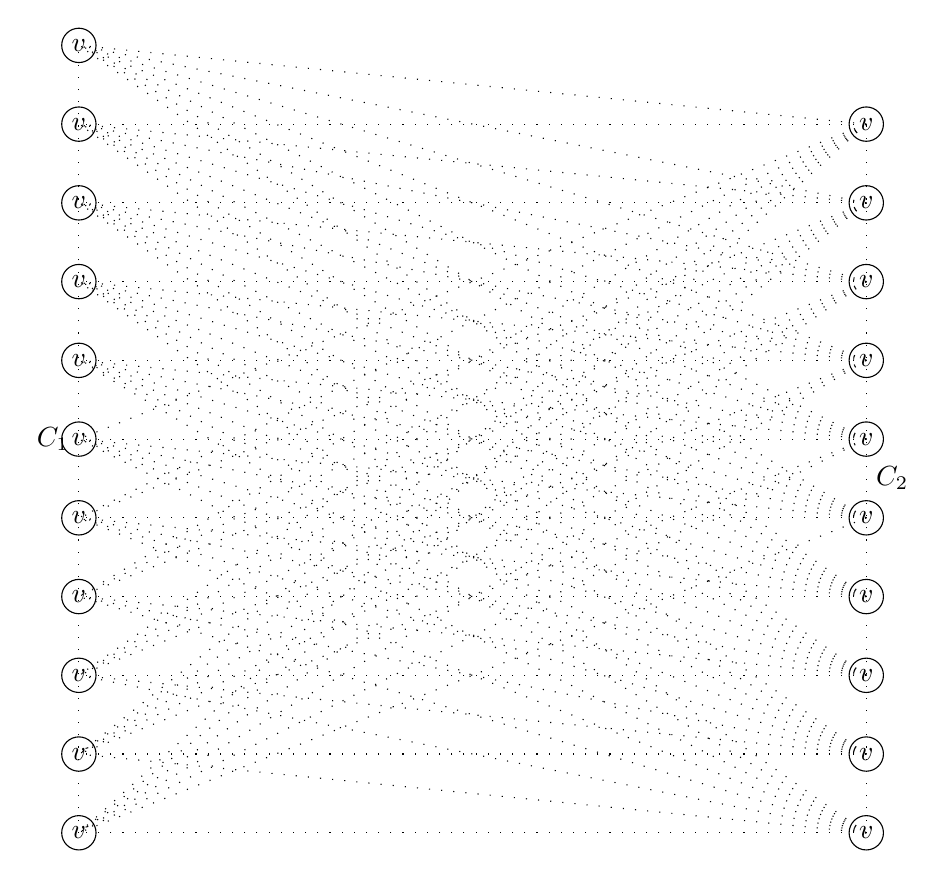
\begin{tikzpicture}
	\def\n{10}
	\def\m{9}
	\pgfmathparse{\m - 2} \let \k \pgfmathresult

	\foreach \y in {0,1,...,\n}{
		\node[draw,circle,inner sep=2pt] at (0, \y) {$v$};
	}

	\foreach \y in {0,1,...,\m}{
		\node[draw,circle,inner sep=2pt] at (10, \y) {$v$};
	}

	\draw[loosely dotted] (0, 0) -- node[left] {$C_1$} (0,\n);
	\draw[loosely dotted] (10, 0) -- node[right] {$C_2$} (10,\m);

	\foreach \x in {0,...,\m}{
		\foreach \y in {0,...,\k}{
			\pgfmathparse{mod(\x + \y, \n + 1)} \let \z \pgfmathresult
			\draw[loosely dotted] (10, \x) -- (0, \z);
		}
	}

	\end{tikzpicture}
\end{slide}


\begin{slide}
	\begin{center}
		{\large Fence graph }
	\end{center}
	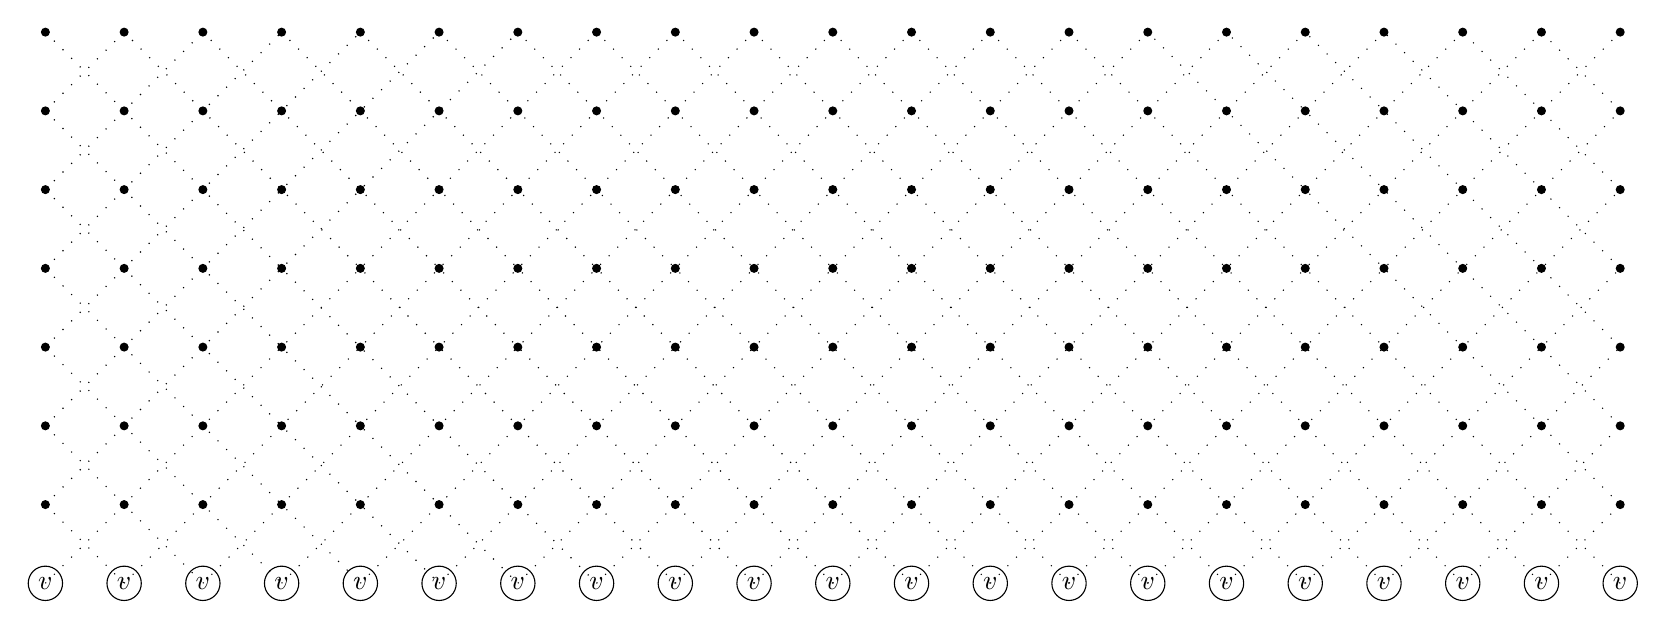
\begin{tikzpicture}
		\def\n{20}
		\def\k{7}
		\pgfmathparse{\n - \k - 1} \let \diff \pgfmathresult
		\foreach \x in {0,1,...,\n}{
			\node[draw,circle,inner sep=2pt] at (\x, 0) {$v$};
			\foreach \y in {1,2,...,\k}{
					\node[draw,circle,inner sep=1pt,fill] at (\x,\y) {};
				}
			}
		\foreach \x in {1,...,\k}{
			\draw[loosely dotted] (0, \k - \x) -- (\x,\k);
			\draw[loosely dotted] (\n - \x, 0) -- (\n, \x);

			\draw[loosely dotted] (0, \x) -- (\x,0);
			\draw[loosely dotted] (\n, \k - \x) -- (\n -\x, \k);
		}
		\foreach \x in {1,...,\diff}{
			\draw[loosely dotted] (\x, 0) -- (\x+\k,\k);
			\draw[loosely dotted] (\n - \x, 0) -- (\n-\x-\k,\k);
		}
	\end{tikzpicture}
\end{slide}


\begin{slide}
	\begin{center}{\large Folding point}\end{center}
	\begin{itemize}
		\setlength{\itemsep}{0pt}
		\setlength{\parskip}{20pt}
		\setlength{\parsep}{0pt}
		\item This is a point where remaining active graph becomes neighborhood graph of one of the processed vertex.
		\item At this point further processing stops.
		\item Folding point could be within the last $K-1$ active vertices; processing stops at $K$ vertices since $K-1$ vertices can't produce clique of size $K$.
	\end{itemize}
\end{slide}


\begin{slide}
	\begin{center}{\large Time complexity when $N < 2k$ having partition extraction applied ahead}\end{center}
	\small
	\begin{itemize}
		\setlength{\itemsep}{0pt}
		\setlength{\parskip}{20pt}
		\setlength{\parsep}{0pt}
		\item This case is considered for set of graphs such that $N < 2k$ where $N = |G|$ and no further partition can be extracted.
		\item Only graphs (non multipartite graph) that can resist partition extraction and satisfies $N < 2k$ would be here.
		\item Removing a vertex that does not have $k$ edges is of $O(n)$. So removing set of vertices that does not have $k$ edges is $O(n\textsuperscript{2})$
		\item Any graph that does not meet edge count criteria will not have clique of size $k$ and the processing stops here. Time complexity is $O(n)$.
		\item Clique sets which resist partition extraction could also satisfy edge count criteria; but they collapse at neighborhood graph processing and after few vertices are processed. Time complexity is polynomial.
		\item If the graph is neither multipartite (friendly to partition extraction) nor clique sets and then they barely meets edge criteria. These graphs mostly have the shape of fence. These graphs collapse at neighborhood graph processing and after few vertices are processed. Time complexity is polynomial.
		\item If the graph is none of the above, then vertex with least degree does not yield a neighborhood graph that could have a clique of $k - 1$. Time complexity is $O(n\textsuperscript{3})$
		\item So, the time complexity for finding clique of $k$ where $N < 2K$ and partitions can not be extracted is polynomial.
	\end{itemize}
\end{slide}


\begin{slide}
	\begin{center}
		{\large Counting \& Enumerating all maximum cliques}
	\end{center}
	\begin{itemize}
		\setlength{\itemsep}{0pt}
		\setlength{\parskip}{5pt}
		\setlength{\parsep}{0pt}
		\item Partition extraction
		\begin{itemize}
			\setlength{\itemsep}{0pt}
			\setlength{\parskip}{5pt}
			\setlength{\parsep}{0pt}
			\item Extracts complete partition
			\item At least one vertex in the partition is connected to all vertices in all other partitions.
			\item Partition may contain one or more vertex that is not connected to all other vertices in other partitions.
		\end{itemize}
		\item When a active vertex's neighborhood graph is explored, a partition is created with the current active vertex. This partition should also contain vertices that have same neighborhood but not connected to active vertex that is being explored.
		\item When a multipartite graph with largest partition is found and there is no more vertex to be explored:
		\begin{itemize}
			\setlength{\itemsep}{0pt}
			\setlength{\parskip}{5pt}
			\setlength{\parsep}{0pt}
			\item Extract proper complete partition. if the vertex that is connected to some of the vertices is not part of the clique then exclude it; otherwise extract a limited complete multipartite graph containing it.
			\item There may be more than one complete multipartite graph.
			\item Number of partitions is nothing but the clique size
			\item Product of each partition size gives number of cliques in that multipartite graph for counting.
			\item Multi-partite graph contains all the cliques that is explored.
		\end{itemize}
		\item Enumerating all multipartite graphs with given number of partitions (maximum clique size) in $G$ gives
			\begin{itemize}
				\setlength{\itemsep}{0pt}
				\setlength{\parskip}{5pt}
				\setlength{\parsep}{0pt}
				\item Total count of maximum cliques.
				\item All maximum cliques (in compressed format : in the form of multipartite graph).
			\end{itemize}
	\end{itemize}
\end{slide}

\begin{slide}
	\begin{center}
		Algorithm enhancements
	\end{center}
	\begin{itemize}
		\setlength{\itemsep}{0pt}
		\setlength{\parskip}{20pt}
		\setlength{\parsep}{0pt}
		\item Find the maximum clique size. 
		\item At least one maximum clique
		\item Count of all maximum cliques present
		\item Enumerate and list all maximum cliques in the form of set of complete multipartite graphs.
	\end{itemize}
\end{slide}


\begin{algorithm}
	\caption{$MaximumClique$ : O(n\textsuperscript{(log(n))})}
	\begin{algorithmic}[1]
		\Function{MaximumClique}{$G(V,E), k, {\color{red} partitions, op}$}
		\State $kMax \gets max(k - 1, 0)$
		\State $H \gets G$
		\While{$(|H| > kMax)$}
		\While{$|(p := ExtractPartition(H))| > 0$}
		\State $partitions \gets partitions \cup p$
		\State $H \gets H - p$
		\State $kMax \gets max(kMax - 1, 0$)
		\EndWhile
		\State
		\If{($H = \{\}$)}
			{\color{red} \If{($kMax = 0$)}
				\State \Comment{Count or Enumerate or etc...}
			\EndIf }
			\State \textbf{break}
		\EndIf
		\State
		\If{($|H| < 2 * kMax$)}
		\algstore{algsave}
	\end{algorithmic}
\end{algorithm}


\begin{algorithm}
	\begin{algorithmic}[1]
		\algrestore{algsave}
		\State $k_1 \gets |H|-kMax$
		\State $E_1 \gets kMax + SumTopVertexEdges(H)$
		\State $E_2 \gets k_1 + SumOtherVertexEdges(H)$
		\If{(($E_1 - kMax^2) < (E_2 - k_1^2$))}
		\State \textbf{break}
		\EndIf
		\EndIf
		\State
		\State $v \gets PickAVertexWithLeastDegree(H)$
		\State {\color{red} $pp \gets partitions \cup \{v, ...\}$ }
		\State $G' \gets neighborhood(H, v, kMax)$
		\If{($|G'| >= kMax$)}
		\State {\color{red} $search \gets (op \textbf{ not in } \{Count, Enumerate\})$ }
		\ForAll {$v' \in \{G - H\}$}
		\State $G'' \gets neighborhood(G, v')$
		\If{($isSubgraph(G'', G')$}
		\State $search \gets false$
		\EndIf
		\EndFor
		\algstore{algsave}
	\end{algorithmic}
\end{algorithm}


\begin{algorithm}
	\begin{algorithmic}[1]
		\algrestore{algsave}
		\If {($search$)}
		\State $(found_1, kMax_1) \gets MaximumClique(G', kMax, {\color{red} pp, op})$
		\If{($found_1$ and (($kMax_1 + 1) > kMax$))}
		\State $kMax \gets kMax_1 + 1$
		\EndIf
		\EndIf
		\EndIf
		\State
		\State $G' \gets neighborhood(H, v)$
		\State $H \gets \{H - v\}$
		
		\ForAll {$v' \in H$}
		\State $G'' \gets neighborhood(H, v')$
		\If{($isSubgraph(G', G'')$}
		\State $H \gets \{H - v'\}$
		\EndIf
		\EndFor
		\EndWhile
		\State $kMax \gets |partitions| + kMax$
		\State \textbf{return} $(kMax >= k, kMax)$
	\EndFunction
	\end{algorithmic}
\end{algorithm}

\clearpage


\begin{slide}
	\begin{center}
		Space complexity in terms of $|G|$
	\end{center}
	\begin{itemize}
		\setlength{\itemsep}{0pt}
		\setlength{\parskip}{20pt}
		\setlength{\parsep}{0pt}
		\item A graph is created at each recursion level. Space requirement for graph is $O(n^2)$. 
		\item At each level fixed set of array is created based on $|G|$. Space requirement is $O(n)$.
		\item Algorithm recursion depth is related to $|G|$. Though recursion depth is related to $|G|$, the actual one is substantially smaller portion of $|G|$.
		\item At each level, input size $n$ is smaller than previous level.
		\item Therefore the space complexity is lower than $O(n^3)$.
	\end{itemize}
\end{slide}


\begin{slide}
	\begin{center}
		Space optimization $|G|$
	\end{center}
	\begin{itemize}
		\setlength{\itemsep}{0pt}
		\setlength{\parskip}{20pt}
		\setlength{\parsep}{0pt}
		\item Though the space complexity is lower than $O(n^3)$, it is still larger than a computer system can provide for when $N$ is in 1000's.
		\item When algorithm runs out of space (RAM), it could free-up top level intermediate graph(s) on need basis. When inner level returns, the freed up graph can be reconstructed from top most level's input graph.
		\item This would avoid flushing RAM contents in to disk storage which is costly in many order of magnitude.
	\end{itemize}
\end{slide}


\begin{slide}
	\begin{center}
		Algorithm sensitivity to CPU data cache.
	\end{center}
	\begin{itemize}
		\setlength{\itemsep}{0pt}
		\setlength{\parskip}{20pt}
		\setlength{\parsep}{0pt}
		\item Access speed of CPU data-cache is many order of magnitude faster than accessing system RAM.
		\item Modern computer(s) have large enough CPU data-cache to handle graph(s) with 100's of vertices without frequently swapping between CPU data-cache and system RAM.
		\item As the $|G|$ size increases, CPU data-cache size is not sufficient enough to hold the entire graph for few levels. At this instance, algorithm speed is entirely depends on the speed of accessing system RAM.
		\item Therefore, the wall clock time to process graphs with 1000's of vertices is many order slower even though the time complexity is same.
	\end{itemize}
\end{slide}


\begin{slide}
	\begin{center}
		Number of proper complete multipartite graphs in G(V,E) relation to $|V|$.
	\end{center}
	\begin{itemize}
		\setlength{\itemsep}{0pt}
		\setlength{\parskip}{5pt}
		\setlength{\parsep}{0pt}
		\item Trivial complete multipartite graph
		\begin{itemize}
			\setlength{\itemsep}{0pt}
			\setlength{\parskip}{00pt}
			\setlength{\parsep}{0pt}
			\item All partitions are trivial. (i.e.) Each partition contains exactly one vertex in it.
			\item Number of cliques in a trivial complete multipartite graph is exactly one.
		\end{itemize}
		\item Proper complete multipartite graph
		\begin{itemize}
			\setlength{\itemsep}{0pt}
			\setlength{\parskip}{00pt}
			\setlength{\parsep}{0pt}
			\item A complete multipartite graph which is not a subgraph of another complete multipartite graph.
			\item There is no other complete multipartite graph which exist can be combined to form a new complete multipartite graph.
		\end{itemize}
		\item Trivial complete multipartite graph can also be a proper complete multipartite graph.
		\item Complexity
		\begin{itemize}
			\setlength{\itemsep}{0pt}
			\setlength{\parskip}{00pt}
			\setlength{\parsep}{0pt}
			\item Fix clique size to K
			\item Partition the set of vertices into two groups.
			\item Take all vertices of one group and create as many proper complete (k-1)-partite graph as possible.
			\item For each vertex in second group, create one trivial k-partite graph from each proper complete k-partite graphs as follows.
			\begin{itemize}
				\setlength{\itemsep}{0pt}
				\setlength{\parskip}{00pt}
				\setlength{\parsep}{0pt}
				\item Create one trivial (k-1)-partite graph from each proper complete (k-1)-partite graph.
				\item the same k-1 partite graph can't be used more than once.
				\item Add the vertex from second group to form a trivial complete k-partite graph.
			\end{itemize}
			\item Since, we can create number of vertices in the second group times number of proper (k-1)-partite graphs, and all are proper complete k-partite graph, complexity is $O(n^2)$
			\item Though the complexity of number of instances is $O(n^2)$, these instances can be packed in $O(n)$ packs.
		\end{itemize}
	\end{itemize}
\end{slide}


\begin{slide}
	\begin{center}
		{\large What is the maximum number of cliques a graph $G(V,E)$ can have and at what clique size? }
	\end{center}
	\begin{itemize}
		\setlength{\itemsep}{0pt}
		\setlength{\parskip}{0pt}
		\setlength{\parsep}{0pt}
		\item $N \bmod 3 \equiv 0$
		\begin{itemize}
			\setlength{\itemsep}{0pt}
			\setlength{\parskip}{0pt}
			\setlength{\parsep}{0pt}
			\item $N/3$ partitions; each having $3$ vertices in it.
			\item Maximum clique size $ : N/3$
			\item Number of cliques with size $N/3$ is $(N/3)^3$
		\end{itemize}
		\item $N \bmod 3 \equiv 1$
		\begin{itemize}
			\setlength{\itemsep}{0pt}
			\setlength{\parskip}{0pt}
			\setlength{\parsep}{0pt}
			\item $((N-1)/3)+1$ partitions; $(N-4)/3$ partitions having $3$ vertices and $2$ partitions having two vertices.
			\item Maximum clique size $ : ((N-1)/3)+1$
			\item Number of cliques with size $((N-1)/3)+1$ is $((N-4)/3)^3 \times 2^2$
		\end{itemize}
		\item $N \bmod 3 \equiv 2$
		\begin{itemize}
			\setlength{\itemsep}{0pt}
			\setlength{\parskip}{0pt}
			\setlength{\parsep}{0pt}
			\item $((N-2)/3)+1$ partitions; $(N-2)/3$ partitions having $3$ vertices and one partition having two vertices.
			\item Maximum clique size $ : ((N-2)/3)+1$
			\item Number of cliques with size $((N-2)/3)+1$ is $((N-2)/3)^3 \times 2$
		\end{itemize}
	\end{itemize}
\end{slide}


\begin{slide}
	\begin{center}
		Time complexity for $G(V, E)$ with $N$ vertices
	\end{center}
	\begin{itemize}
		\setlength{\itemsep}{0pt}
		\setlength{\parskip}{10pt}
		\setlength{\parsep}{0pt}
		\item For worst case analysis, we take maximum clique size $K$ is same as number of partition $P$. If the $K$ is lower than $P$ then it has lower time complexity compared to where $K = P$.
		\item Number of partitions ($P$) in the graph: this determines the maximum size of the clique. Also determines the depth the iterations.
		\item Partition size ($S$): Minimum partition size is 1; maximum possible partition size is ($N - P + 1$)
		\item Sum of vertices in all partitions equals $N$.
		\item Average partition size is $N / P$
		\item At each iteration, we only need to explore ($N_i - 2 * K_i + 1$).
		\item At each depth or partition extraction, $K_i$ gets reduced by $1$ while $N_i$ gets reduced by at least $3$.The iteration size reduces acutely.
		\item Further exploring is needed until $N_i$ becomes lesser than $2K_i$. At this point, remaining processing becomes polynomial.
		\item As vertices are processed and removed from active consideration, the remaining active graph becomes smaller, and starts exposing multi-partite graphs. This enables both partition extraction and neighborhood graph duplicate removal optimization to take place.
		\item Both number of partitions $P$ and average partition size $S$ are controlled by $N$ as $P * S = N$.
		\item $K$ is directly proportional to $P$.
		\item $K$ is inversely proportional to $S$.
		\item Folding point's location at each depth; Pushing folding point to within $2K-1$ at each depth makes the overall depth shallow due acute convergence.
		\item Larger $P$
		\begin{itemize}
			\setlength{\itemsep}{0pt}
			\setlength{\parskip}{5pt}
			\setlength{\parsep}{0pt}
			\item As the $P$ increases, $K_i$ at each level also increases.
			\item It is only ($N_i - 2 * K_i + 1$) needs to processed at each level, therefore the number of vertices needs to be explored becomes smaller at each level.
			\item Larger $K$ requires each vertex to have larger number of edges. This causes convergence towards neighborhood graph with $2K_i$ vertices acute.
			\item Also gap between $N_i$ and $2K_i$ is smaller; so the convergence towards neighborhood graph with $2K_i$ vertices is acute.
			\item Large $K$ means smaller $S$; smaller $S$ brings folding point sooner than $2K_i$. This reduces the number of vertices that needs to be explored at each level.
		\end{itemize} 
		\item Smaller $P$
		\begin{itemize}
			\setlength{\itemsep}{0pt}
			\setlength{\parskip}{5pt}
			\setlength{\parsep}{0pt}
			\item As the $P$ decreases, the required depth of the search decreases.
			\item With larger partition size $S$, subsequent neighborhood graph becomes smaller and smaller acutely.
			\item If the graph $G$ is denser then both partition extraction and neighborhood graph elimination (bottom up processing) works aggressively.
			\item If the graph is sparse then it has lower time complexity.
		\end{itemize} 
		\item $P \approx S$
		\begin{itemize}
			\setlength{\itemsep}{0pt}
			\setlength{\parskip}{5pt}
			\setlength{\parsep}{0pt}
			\item Sufficient enough depth to provide maximum possible breath at each level.
			\item Even at this parameters, the convergence to neighborhood graph of $2K_i$ is acute; does not require to explore to the depth of $K$.
			\item Simplistic order here is $O(N^{\sqrt{N}-C})$ where $C > 0$.
			\item Since number of vertices explored at each level is at least $S$ lower than then previous level, the above time complexity can be rewritten as $O(N^{k(\sqrt{N} - C)})$ where $C > 0$ and $0 < k < 1$. As $C$ increases $k$ tends towards $1$ and vice versa.
		\end{itemize} 
	\end{itemize}
\end{slide}


\begin{slide}
	\begin{center}
		Observed Time complexity for $G(V, E)$ with $N$ vertices
	\end{center}
	\begin{itemize}
		\setlength{\itemsep}{0pt}
		\setlength{\parskip}{10pt}
		\setlength{\parsep}{0pt}
		\item $C$ in the above time complexity reaches more than half of $\sqrt{N}$.
		\item For a graph $G(V,E)$ with 512 vertices, the time complexity is coming around $O(N^6)$. That is roughly around $O((2^9)^6)$ = $O(2\textsuperscript{54})$.
	\end{itemize}
\end{slide}


\begin{slide}
	\begin{center}
		Minor optimization
	\end{center}
	\begin{itemize}
		\setlength{\itemsep}{0pt}
		\setlength{\parskip}{10pt}
		\setlength{\parsep}{0pt}
		\item Let $v^1$ \& $v^2$ are vertices of graph $G$.
		\item Let $G^1$ be neighborhood graph of $v^1$.
		\item Let $G^2$ be neighborhood graph of $v^2$.
		\item Let $S^1$ is set of vertices found only in $G^1$.
		\item Let $S^2$ is set of vertices found only in $G^2$.
		\item Let $S'$ is set of vertices found in both $G^1$ \& $G^2$.
		\item Consider that $G^1$ is already explored.
		\item During the processing of $G^2$, we can discard any graph $G''$ which has all vertices from $S'$. This is because, $G''$ is already explored as part of $G^1$.
	\end{itemize}
\end{slide}


\begin{slide}
	\begin{center}
		Execution statistics for keller5.clq \\
		http://mat.gsia.cmu.edu/COLOR02/INSTANCES/keller5.clq \\
	\end{center}
	\begin{tabular}{ l r }
		Vertices & 776 \\
		Edges & 225990 \\
		Clique & 27 \\
		Ticks(ms) & 2542521999 \\
		Calls & 703285173499 \\
		TwoNHits & 633190806735 \\
		SubgraphHits & 1179362341357 \\
		BtmUpHits & 495495356392 \\
		BtmUpHits2 & 1317047970 \\
	\end{tabular}
	\\ \\ \\
	\begin{tabular}{ r r }
		Depth &		 Calls \\
		1 &               1 \\
		2 &             401 \\
		3 &          142948 \\
		4 &        18402772 \\
		5 &      1047840586 \\
		6 &     26427005000 \\
		7 &    249569092300 \\
		8 &    400189686052 \\
		9 &     26026406477 \\
		10 &        6596962  \\
	\end{tabular}
\end{slide}


\end{document}
